\documentclass{report}
\usepackage{blindtext}
\usepackage[T1]{fontenc}
\usepackage[utf8]{inputenc}
\usepackage{listings}


\title{POS Projekt}
\author{Alessandro Crispino}
\date{April 2020}

%\usepackage{natbib}
\usepackage{graphicx}

\begin{document}

\maketitle
\tableofcontents

%includes
%\include{sections/einleitung}

%\bibliographystyle{plain}
%\bibliography{references}

\chapter{Einleitung}
Dieses Projekt wurde im Zuge der Aubesserung der POS-Note durchgeführt. Die Aufgabe war es einen Bankomaten, wie er in Österreich existiert, mittels der Library ``[Boost].SML`` zu implementieren. Dafür wurde zuerst ein UML-Zustandsdiagramm erstellt und dieses anschliessend mittels ``[Boost].SML`` umgesetzt.


\chapter{[Boost].SML}
\begin{figure}[h]
  \centering
  
\includegraphics[scale=0.5]{images/boost.png}
  \caption[Logo]{Logo [Boost].SML} 
\end{figure}

Bei [Boost].SML handelt es sich handelt es sich um eine skalierbare header-only State Machine Library. Mittels dieser Bibliothek soll es ermöglicht werden unstrukturierten und unleserlichen Code zu verbessern. [Boost].SML ist ausserdem eine Verbesserung des Vorgängers Boost.MSM, welcher einige Nachteile hatte. Somit kann man [Boost].SML auch als Verbesserung von Boost.MSM definieren. [Boost].SML kann ab C++14 verwendet werden.

\section{Installation}
Um [Boost].SML verwenden zu können muss die Library zuerst installiert werden. Da es sich hierbei um eine header-only Library handelt, muss diese nur mit folgendem Kommando heruntergeladen werden:
\newline
wget https://raw.githubusercontent.com/boost-experimental/sml/master/include/boost/sml.hpp
\newline
\vspace{5mm}
Anschliessend muss die Header Date eingebunden und der ``sml`` namespace definiert werden. Dies funktioniert folgendermaßen:
\begin{lstlisting}[language=C++]
#include "boost/sml.hpp"
namespace sml = boost::sml;
\end{lstlisting}
Wichtig ist noch zu erwähnen, dass [Boost].SML erst ab C++14 verwendet werden kann. 

\section{Features}
Im folgenden Abschnitt werden die einzelnen Funktionen und Elemente der Bibliothek aufgezählt und erklärt.

\subsection{States / Zustände und Events / Ereignis}
Ein endlicher Automat besteht aus einer endlichen Anzahl von Zuständen und Übergängen. Diese Übergänge werden durch Ereignisse ausgelöst. Daher handelt es sich bei States und Events um Grundelemente der Library. 

\subsubsection{Implementierung States}
States werden folgendermaßen implementiert: 
\begin{lstlisting}[language=C++]
auto Automat_Bereit_state = "Automat_Bereit"_s;
\end{lstlisting}
Ausserdem können Endzustände festgelegt werden welche folgend implementiert werden:
\begin{lstlisting}[language=C++]
"Automat_Bereit"_s = X;
\end{lstlisting}
Zustände können zudem folgendermaßen ausgegeben werden:
\begin{lstlisting}[language=C++]
std::cout << state.c_str() << std::endl;
\end{lstlisting}

\subsubsection{Implementierung Events}
Events können folgendermaßen implementiert werden:
\begin{lstlisting}[language=C++]
struct Karte_Einfuehren_event{};
\end{lstlisting}

\subsection{Guards und Actions}
Bei Guards und Actions handelt es sich um aufrufbare Objekte welche vom Automaten ausgeführt werden um zu überprüfen ob ein Übergang stattfinden soll. Guards müssen hierbei einen booleschen Wert zurückliefern. Actions hingegen müssen keine Rückgabewert besitzen.

\subsubsection{Implementierung Guards}
Guards können wie folgt implementiert werden:
\begin{lstlisting}[language=C++]
const auto geldentnahme = []() {
    //Code
    return true;
};
\end{lstlisting}

\subsubsection{Implementierung Actions}
Actions werden ähnlich wie Guards erstellt allerdings müssen diese, wie bereits erwähnt, nichts zurückgeben. Ausserdem können diese auch mittels Lambda Ausdrücken im Transition Table implementiert werden. Dies sieht folgendermaßen aus:
\begin{lstlisting}[language=C++]
event<name\_event> / [] { cout << ``Karte wird eingeführt`` < endl; }
\end{lstlisting}
Dazu später mehr
%vielleicht unterpunkt dann verlinken

\subsection{Transition Table}
Um States, Events, Guards und Actions zu verbinden wird ein Transition Table benötigt. Dieser verbindet alle oben erwähnten Elemente und bildet daraus einen Automaten. Ein Transition Table kann folgendermaßen aussehen:
\begin{lstlisting}[language=C++]
using namespace sml;

make_transition_table(
 *"src_state"_s + event<my_event> [ guard ] / action = "dst_state"_s
, "dst_state"_s + "other_event"_e = X
);
\end{lstlisting}
\vspace{5mm}
Ausserdem können bei der Implementierung eines solchen Tables zwei verschiedene Notationen verwendet werden, diese sind die Postfix und Prefix Notation. 
\newline
Die folgende Auflistung zeigt die verschiedenen Funktion, in den verschiedenen Notationen:

\textbf{Postfix:}
\begin{itemize}
    \item Übergang Zustand und Event mit Guard: \newline state + event [ guard ]
    \item anonymer Übergang mit Action: \newline src\_state / [] {} = dst\_state
    \item Selbstübergang: \newline src\_state / [] {} = src\_state
    \item Übergang ohne Guard oder Action: \newline src\_state + event = dst\_state
    \item Übergang mit Guard und Action: \newline src\_state + event [ guard ] / action = dst\_state	
    \item Übergang mit mehreren Guards und Actions: \newline src\_state + event [ guard \&\& (![]{return true;} \&\& guard2) ] / (action, action2, []{}) = dst\_state	
\end{itemize}

\textbf{Prefix:}
\begin{itemize}
    \item Übergang Zustand und Event mit Guard: \newline state + event [ guard ]
    \item anonymer Übergang mit Action: \newline dst\_state <= src\_state / [] {}
    \item Selbstübergang: \newline src\_state <= src\_state / [] {}
    \item Übergang ohne Guard oder Action: \newline dst\_state <= src\_state + event
    \item Übergang mit Guard und Action: \newline dst\_state <= src\_state + event [ guard ] / action
    \item Übergang mit mehreren Guards und Actions: \newline dst\_state <= src\_state + event [ guard \&\& (![]{return true;} \&\& guard2) ] / (action, action2, []{})
\end{itemize}

\subsection{Startzustände}
Da jeder Automat an einem bestimmten Punkt beginnen muss gibt es Startzustände. Diese definieren den Anfang eines Automaten. Startzustände werden mittels eines Sternchens ``*`` implementiert. Dies sieht folgendermaßen aus:
\begin{lstlisting}[language=C++]
return make_transition_table(
    *start\_state + event<name\_event> = end\_state
);
\end{lstlisting}

\subsection{State Machine}
%4Methoden noch Zeigen
Um eine State Machine zu erstellen wird ein Transition Table benötigt. Dieser Transition Table wird mittels der Funktion ``make\_transition\_table`` in einem überladenen Operator ``()`` einer Klasse erstellt. Dies sieht folgendermaßen aus:
\begin{lstlisting}[language=C++]
class test {
public:
  auto opeartor()() {
    using namespace sml;
    return make_transition_table(
     *"src_state"_s + event<my_event> [ guard ] / action = "dst_state"_s,
      "dst_state"_s + event<game_over> = X
    );
  }
};
\end{lstlisting}
Mittels folgendem Code wird anschließend eine State Machine erzeugt:
\begin{lstlisting}[language=C++]
sml::sm<test> sm;
\end{lstlisting}
Ausserdem können den Guards und Actions Parameter mittels des Konstruktors übergeben werden. Um dies besser nachvollziehen zu können, dient folgendes Code-Beispiel:
\begin{lstlisting}[language=C++]
auto guard = [](double d) { return true; }
                   |
                   \--------\
                            |
auto action = [](int i){}   |
                  |         |
                  |         |
                  \-\   /---/
                    |   |
sml::sm<example> s{42, 87.0};
\end{lstlisting}

\subsection{Events ausführen}
Um einen Automaten verwenden zu können, müssen die einzelnen Events ausgeführt werden. Ist dies im Transition Table richtig definiert so gelangt man von einem Zustand mittels der Ausführung eines Events in den nächsten. Dafür gibt es die Methode ``process\_event``. Diese wird folgendermaßen verwendet:
\begin{lstlisting}[language=C++]
sml::sm<example> sm;

sm.process_event(event{});
\end{lstlisting}
Events können außerdem auch im Transition Table ausgelöst werden. Das wird wie folgt gemacht:
\begin{lstlisting}[language=C++]
start_state + event<my_event> / process(my_event_to_process{}) = end_state
\end{lstlisting}

\subsection{Fehlerbehandlung}
Falls es zu dem Fall kommen sollte, dass eine State Machine ein ausgelöstes Event nicht behandeln kann, kommt es zu einem ``unexpected event``. Ein solches kann auf folgende Weise abgefangen werden: 
\begin{lstlisting}[language=C++]
"start_state"_s + unexpected_event<some_event> = X
\end{lstlisting}
Ausserdem können auch unbekannte Events mit folgendem Code abgefangen werden:
\begin{lstlisting}[language=C++]
"start_state"_s + unexpected_event<_> = X
\end{lstlisting}
\subsection{Testen}
Um den Automaten auch während des Erstellens testen zu können werden folgende Methoden bereitgestellt:
\begin{itemize}
    \item state\_machine.is: prüfen ob state\_machine im angegebenen Zustand ist
    \item state\_machine.set\_current\_states: setzt den derzeitigen Zustand der state\_machine in den angegebenen Zustand
    \item state\_machine.visit\_current\_states: gibt den derzeitigen Zustand der state\_machine zurück
\end{itemize}

%Dann schreiben wie man das implementiert hat

%Guard -> checken ob event gültig ist
%so: 
%PIN_Aufforderung_state + PIN_Eingabe_event [right_PIN] = Menue_state,
%PIN_Aufforderung_state + PIN_Eingabe_event [!right_PIN] = %Karte_Einziehen_state,

%struct PIN erstellen mit value
%guard erstellenn wo gecheckt wird ob die PIN richtig ist
%PIN anlegen
%in statemachine deklaration übergeben
%vor dem process PIn Eingabe event setzen mit user input
\chapter{Bankomat}
Im folgenden Kapitel wird sich genauer mit der Implementierung des Bankomaten auseinandergesetzt. Hierfür wird zuerst das UML-Zustandsdiagramm gezeigt und anschließend die einzelnen Schritte der Implementierung erklärt.

\section{UML-Zustandsdiagramm}
\begin{figure}
  \centering
  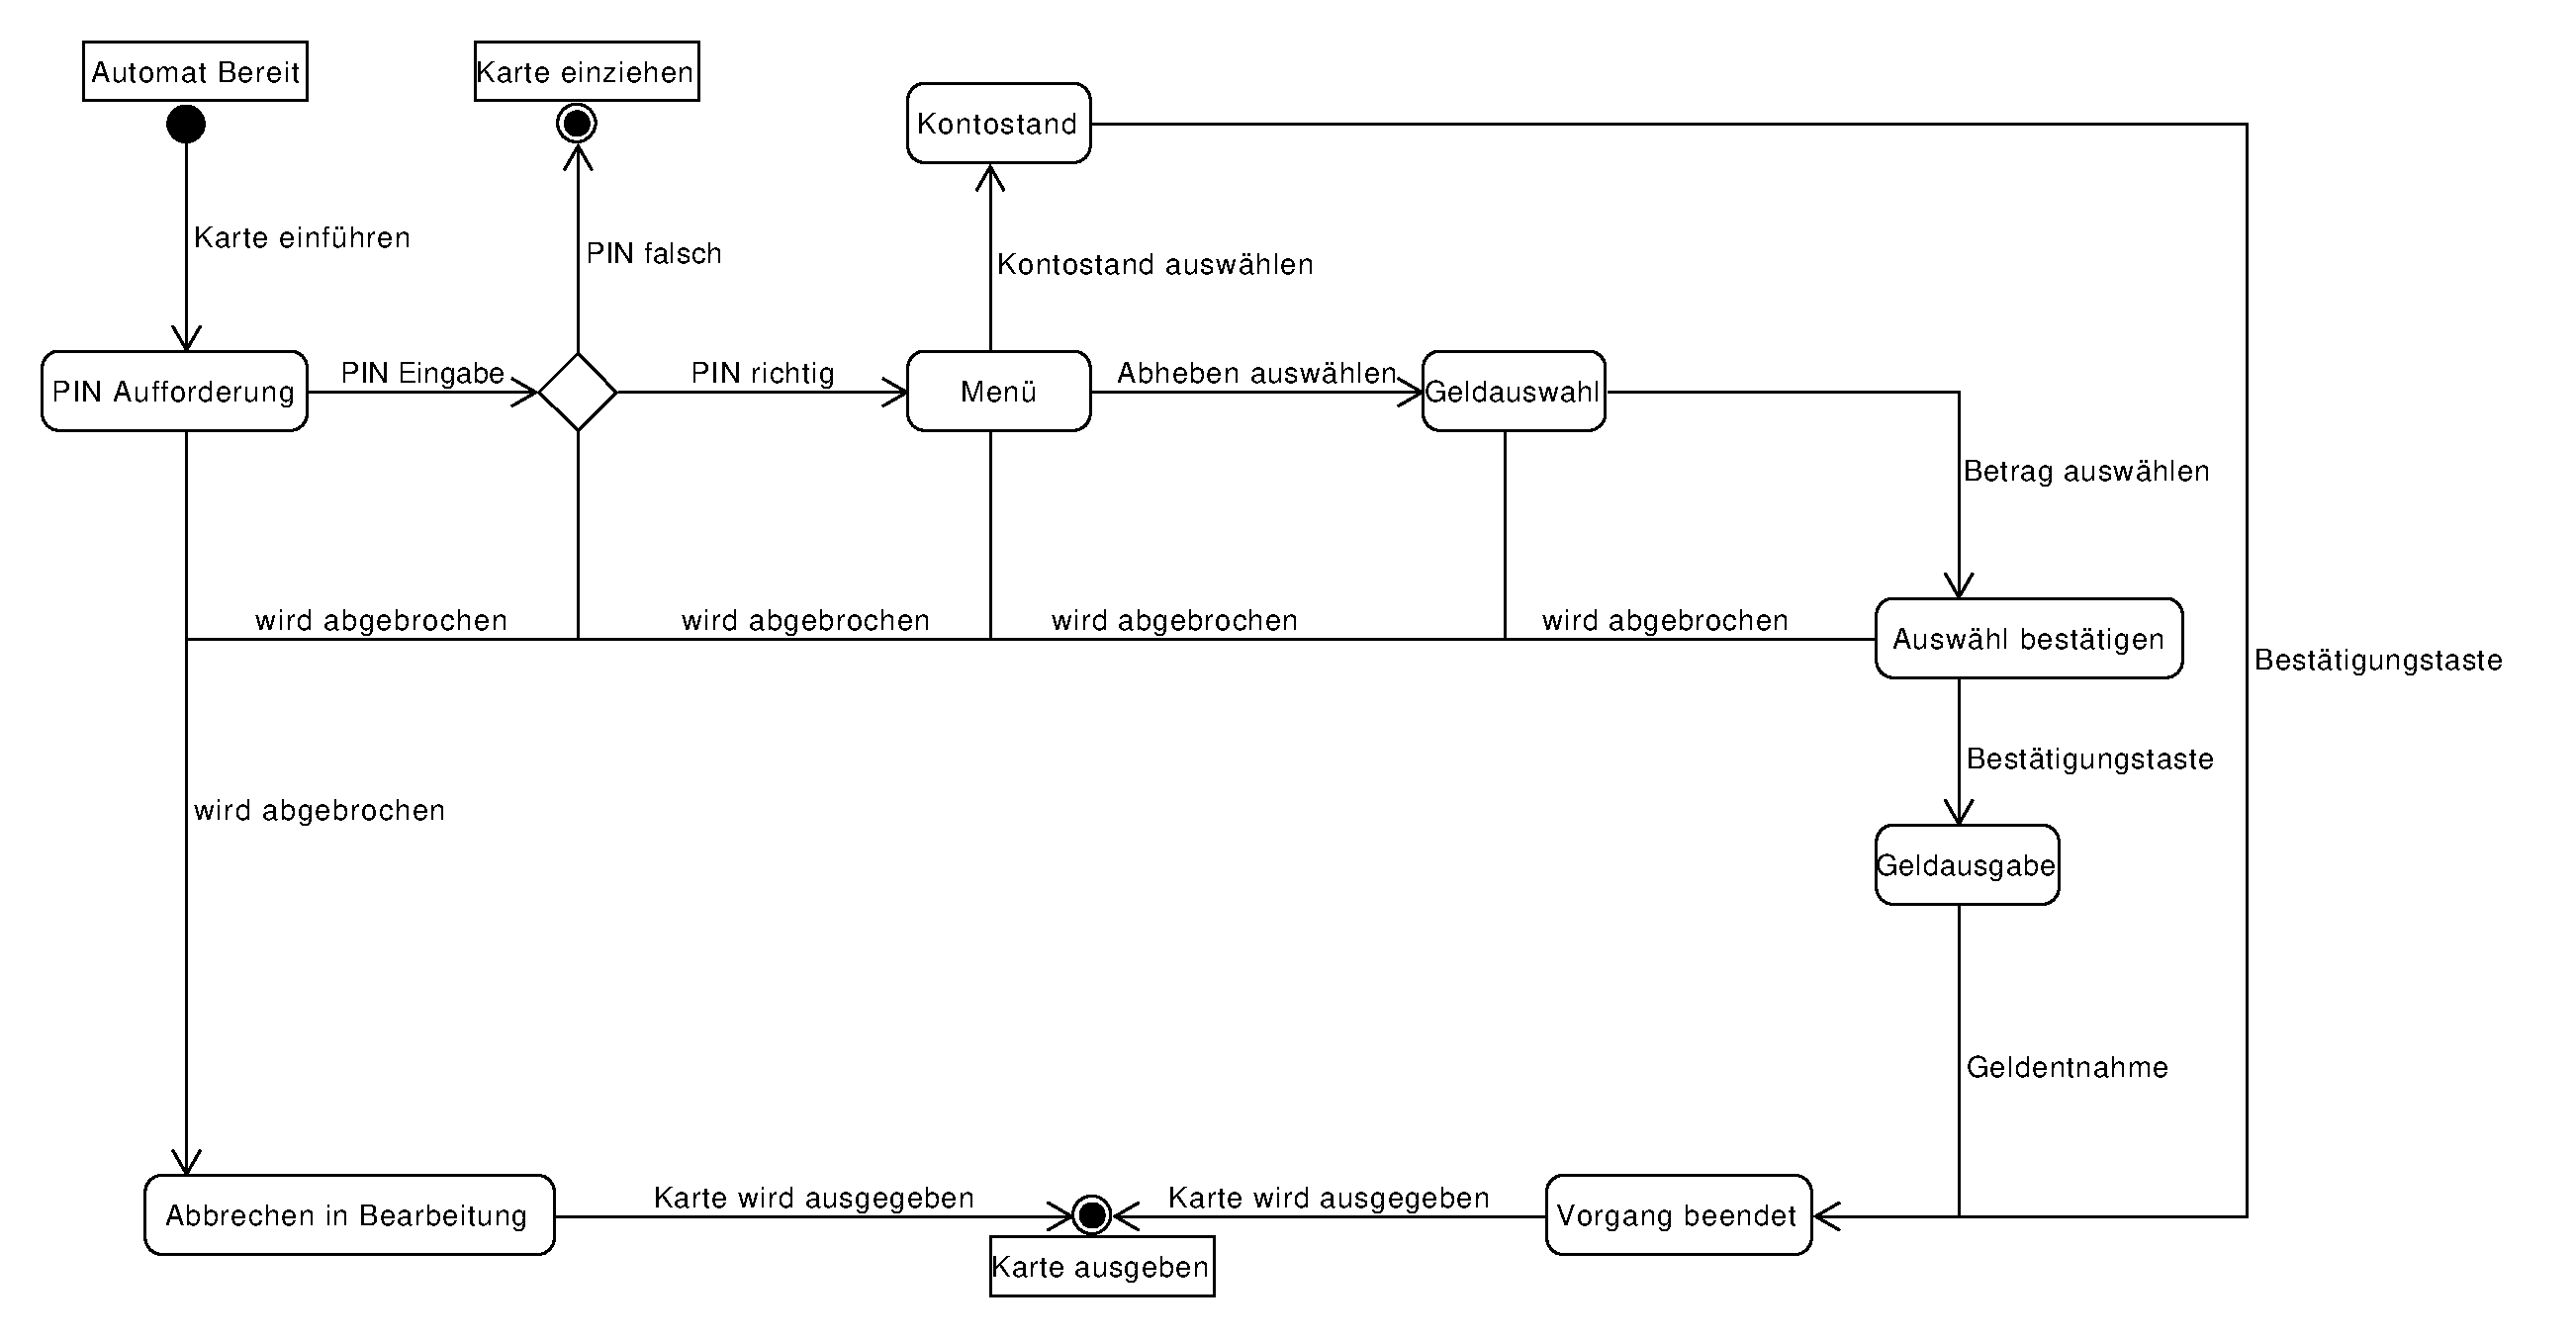
\includegraphics[angle=-90, scale=0.44]{images/zustandsdiagramm_v2.pdf}
  \caption[Bankomat]{Zustandsdiagramm Bankomat} 
\end{figure}

Die Rechtecke mit den abgerundeten Ecken definieren die einzelnen Zustände, Übergänge werden mittels der Pfeile beschrieben. Ausserdem gibt es noch Start- und Endereignisse diese werden durch Kreise charakterisiert. Wobei ein Startereignis aus einem ausgefüllten Kreis besteht und ein Endereignis aus zwei ineinander liegenden Kreisen, wobei der Innere ausgefüllt wird.

\section{Implementierung}
%neues Modul erstellt
\subsection{Grundaufbau}
Zuerst wurde ein neues Modul mit dem Namen ``bankomat.cpp`` und der dazu gehörigen Header Datei angelegt. Der Bankomat wurde ausschließlich in diesem Modul erstellt. Ausserdem wurde ein eigener Namespace mit der Bezeichnung bankomat definiert.


%alle States definiert
\subsection{States}
Im nächsten Schritt wurden alle Zustände des Zustandsdiagramms definiert. Dies wurde auf folgende Weise gemacht:
\begin{lstlisting}
auto machine_ready_state = "Automat_Bereit"_s;
auto pin_request_state = "PIN_Aufforderung"_s;
auto menue_state = "Menue"_s;
auto bank_balance_state = "Kontostand"_s;
auto money_selection_state = "Geldauswahl"_s;
auto confirm_selection_state = "Auswahl_Bestaetigen"_s;
auto money_output_state = "Geldausgabe"_s;
auto withdraw_card_state = "Karte_Einziehen"_s;
auto cancel_in_progress_state = "Abbrechen_In_Bearbeitung"_s;
auto operation_ended_state = "Vorgang_Beendet"_s;
\end{lstlisting}
%alle Events definiert
\subsection{Events}
Nachdem alle States definiert worden sind, sind anschließend alle Events definiert worden. Dies wurde folgendermaßen gemacht:
\begin{lstlisting}
struct input_card_event{};
struct input_pin_event{};
struct select_balance_event{};
struct select_withdraw_event{};
struct confirm_event{};
struct confirm_amount_event{};
struct withdraw_money_event{};
struct cancel_event{};
struct card_output_event{};
\end{lstlisting}
%transition table definiert
\subsection{Transition Table}
Um das ganze letztendlich verbinden zu können wurde eine Transition Table angelegt welcher die Logik des Automaten implementierte. Zudem wurden Guards und Actions angelegt. Dies wurde auf folgende Weise implementiert:
\begin{lstlisting}
return make_transition_table(
    *machine_ready_state + 
        event<input_card_event> 
            / [] { cout << "Karte wird eingefuehrt" << endl; } 
                = pin_request_state,

    pin_request_state + 
        event<input_pin_event>[right_PIN] 
            / [] { cout << "PIN ist richtig" << endl; } 
                = menue_state,

    pin_request_state + 
        event<input_pin_event>[!right_PIN] 
            / [] { cout << "PIN ist falsch, Karte wird eingezogen" << endl; } 
                = withdraw_card_state,

    pin_request_state +
        event<cancel_event> 
        = cancel_in_progress_state,

    menue_state + 
        event<select_balance_event> 
            / [] { cout << "Option Kontostand wurde gewaehlt" << endl; } 
                = bank_balance_state,

    menue_state 
        + event<select_withdraw_event> 
            / [] { cout << "Option Abheben wurde gewaehlt" << endl; } 
                = money_selection_state,
    menue_state 
        + event<cancel_event> 
            / [] { cout << "Vorgang wird abgebrochen" << endl; } 
                = cancel_in_progress_state,

    bank_balance_state 
        + event<confirm_event> 
            / [] { cout << "Option wurde bestaetigt" << endl; } 
                = operation_ended_state,

    money_selection_state 
        + event<confirm_amount_event> 
            = confirm_selection_state,

    money_selection_state 
        + event<cancel_event> 
            / [] { cout << "Vorgang wird abgebrochen" << endl; } 
                = cancel_in_progress_state,

    confirm_selection_state 
        + event<confirm_event> 
            / [] { cout << "Auswahl bestaetigen" << endl; } 
                = money_output_state,

    confirm_selection_state 
        + event<cancel_event> 
            / [] { cout << "Vorgang wird abgebrochen" << endl; } 
                = cancel_in_progress_state,

    money_output_state 
        + event<withdraw_money_event>[withdraw] 
            / process(card_output_event{}) 
                = operation_ended_state,

    operation_ended_state 
        + event<card_output_event> 
            / [] { cout << "Karte wird ausgegeben" << endl; } 
                = X,

    cancel_in_progress_state 
        + event<card_output_event> 
            / [] { cout << "Karte wird ausgegeben" << endl; } 
                = X
);
\end{lstlisting}
Hier wurde jeweil ein Ausganszustand mit einem Event verbunden. Dies resultierte anschließend in einem weiteren Zustand. Guards wurden mittels eckiger Klammern aufgerufen. Actions wurden mittels Lambda Aufrufen realisiert, dafür wurde lediglich nach dem ``/`` ein Lambda Ausdruck definiert. Ausserdem wurde der Startzustand mittels eines Sternchens am Anfang, und ein Endzustand mittels eines ``X`` definiert.
%PIN definiert
\subsection{PIN}
Um es zu ermöglichen den Pin zu überprüfen wurde eine Struktur PIN erstellt. Diese wurde lediglich verwendet um einen Wert und zwar die richtige Zahlenkombination, zu speichern. Die Struktur war wie folgt aufgebaut:
\begin{lstlisting}
struct PIN{
    std::string value{};
};
\end{lstlisting}
%guards definiert
%start Methode
%Pin angelegt sm angelegt
%Eingabe
%Menü
%Kontostand
%Geld abheben

\end{document}
